\documentclass[8pt]{article}
\usepackage{polski}
\usepackage[utf8]{inputenc}
\usepackage{geometry}
\usepackage[argument]{graphicx}
\usepackage{graphicx}
\graphicspath{{images/}{images2/}}
\setlength\fboxsep{3pt}
\setlength\fboxrule{1pt}
\usepackage{pdfpages}
\usepackage{fancyvrb}
\usepackage[pdftex,
pdfauthor={jeleniep},
pdftitle={Opis},
pdfsubject={System do zarządzania publikacjami naukowymi},
pdfkeywords={Some Keywords},
pdfproducer={Latex with hyperref, or other system},
pdfcreator={pdflatex, or other tool}]{hyperref}
\newenvironment{centermath}
{\begin{center}$\displaystyle}
	{$\end{center}}

\begin{document}
	\begin{titlepage}
		\begin{center}
			\Large
			Politechnika Warszawska 
			
			Wydział Elektryczny 
			
			Kierunek Informatyka Stosowana
			\vfill
			\Huge \textsc{Opis systemu  do zarządzania publikacjami naukowymi}
		\end{center}
		\vfill
		
		
		
		\begin{center}
			\Large Piotr Jeleniewicz
			
			nr indeksu 291072
		\end{center}
		
		
		
		
	\end{titlepage}
	\large\tableofcontents
	\Large
	\newpage

	
	\section {Wstęp}
		\hspace{10pt} W ramach projektu dyplomowego wykonany zostanie system do zarządzania publikacjami naukowymi, który będzie automatycznie dokonywał analizy plików PDF. Będzie się on składał z aplikacji serwerowej służącej do analizy plików oraz osbsługi bazy danych, która napisana będzie przy użyciu Node.js oraz języka TypeScript, a także aplikacji klienckiej pracującej na urządzeniach z systemem Android napisanej w języku Kotlin.
	\section {Opis działania}
		\hspace{10pt} Po zainstalowaniu aplikacji na urządzeniu z systemem Android oraz jej uruchomieniu, użytkownik zostanie poproszony o zalogowanie się lub utworzenie konta. Po zalogowaniu, użytkownika będzie miał możliwość tworzenia nowych publikacji, edytowania istniejących oraz wyszukiwania innych użytkowników oraz ich publikacji. 
	\section {Analiza funkcjonalna}	
	\hspace{10pt} 	System będzie udostępniał następujące funkcjonalności:		\begin{enumerate}
		\item Wyświetlanie publikacji naukowych.
		\item Wyszukiwanie publikacji naukowych na podstawie autorów oraz nazwy.
		\item Tworzenie nowej publikacji w oparciu o metadane dostępne w pliku PDF.
		\item Obserwowanie innych użytkowników.
		\item Edycja publikacji.
		\item Wysyłanie powiadomień o nowo dodanej publikacji do osób obserwujących autora publikacji.
		\item Możliwość komentowania publikacji.
		\item Komunikacja tekstowa z innymi użytkownikami systemu.
				
	\end{enumerate}
	\section {Architektura techniczna}	
	\subsection{Diagram komponentów}
	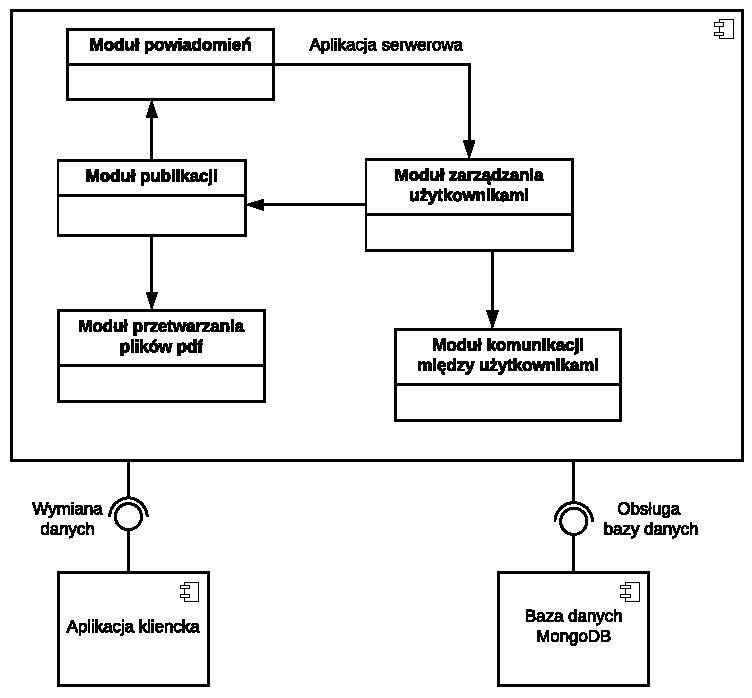
\includegraphics[scale=1.191]{Diagram_komponentow_inz.pdf}
	\subsection{Opis aplikacji serwerowej}
		\hspace{10pt} Aplikacja serwerowa zostanie wykonana przy następujących założeniach:
	\begin{enumerate}
		\item Wykorzystany zostanie framework Node.js oraz język TypeScript.
		\item Aplikacja będzie udostępniać REST Api do komunikacji z aplikacją kliencką.
		\item Wraz bazą danych będzie uruchamiana w środowisku Docker.
		\item Do przechowywania danych wykorzystana zostanie baza danych MongoDB.
		\item Będzie się składać z następujących modułów:
		\begin{enumerate}
			\item moduł zarządzania użytkownikami - odpowiedzialny za rejestrację i logowanie użytkowników,
			\item moduł komunikacji między użytkownikami - odpowiedzialny za wysyłanie wiadomości pomiędzy użytkownikami aplikacji,
			\item moduł publikacji - odpowiedzialny za dodawanie, edycję oraz usuwanie aplikacji,
			\item moduł przetwarzania plików pdf - odpowiedzialny za analizę metadanych plików pdf i tworzeniu na ich podstawie opisu publikacji,
			\item moduł powiadomień - odpowiedzialny za wysyłanie powiadomień do użytkowników,					
		\end{enumerate}		
		\item System będzie zachowywał standardy bezpieczeństwa takie jak wykorzystanie protokołu HTTPS zamiast HTTP oraz walidacja danych otrzymanych w żądaniach.
	\end{enumerate}

	\subsubsection{Metody analizy plików PDF}
		\hspace{10pt} Jedną z najistotniejszych funkcji tego systemu będzie analiza plików PDF w celu pobrania z nich metadanych określających informacje takie jak tytuł czy autor. 
		Przetestowane zostały następujące rozwiązania:
			\begin{enumerate}
			\item Moduł \textit{pdf-parser} - moduł najpopularniejszy ze wszystkich analizowanych, ale też nie rozwijany od 2 lat;
			\item Moduł \textit{pdfreader} - moduł najmniej popularny ze wszystkich analizowanych, wciąż rozwijany;
			\item Moduł \textit{pdf2json} - moduł dość popularny, wciąż rozwijany;
		\end{enumerate}
		\hspace{10pt} Podjęta została próba z wykorzystaniem każdego z modułów. Niestety moduły \textit{pdfreader} oraz \textit{pdf2json} pozbawione są typów, wykrozystywanych w języku TypeScript, w którym tworzona będzie aplikacja serwerowa. Dlatego też do analizy plików pdf wykorzystany zostanie moduł \textit{pdf-parser}, który posiada pełne wsparcie typów w języku TypeScript. Za pomocą tego modułu, uzyskujemy informacje o pliku pdf takie jak tytuł, autor, i inne związane z wersją pdf czy słowami kluczowymi. Umożliwa on także odczyt tekstu z pliku pdf, co może być przydatne do tworzenia skrótów zawierających wstęp pliku. 

	\subsection{Opis aplikacji klienckiej(mobilnej)}
	\hspace{10pt} Aplikacja kliencka zostanie wykonana jako aplikacja mobilna przy następujących założeniach:
	\begin{enumerate}
		\item Aplikcja będzie pracować na systemie Android.
		\item Wykorzystany zostanie język Kotlin.
		\item Wraz bazą danych będzie uruchamiana w środowisku Docker.
		\item Do obsługi powiadomień wykorzystany zostanie Firebase Cloud Messaging.
	\end{enumerate}



\end{document}
